\documentclass[]{book}
\usepackage{lmodern}
\usepackage{amssymb,amsmath}
\usepackage{ifxetex,ifluatex}
\usepackage{fixltx2e} % provides \textsubscript
\ifnum 0\ifxetex 1\fi\ifluatex 1\fi=0 % if pdftex
  \usepackage[T1]{fontenc}
  \usepackage[utf8]{inputenc}
\else % if luatex or xelatex
  \ifxetex
    \usepackage{mathspec}
  \else
    \usepackage{fontspec}
  \fi
  \defaultfontfeatures{Ligatures=TeX,Scale=MatchLowercase}
\fi
% use upquote if available, for straight quotes in verbatim environments
\IfFileExists{upquote.sty}{\usepackage{upquote}}{}
% use microtype if available
\IfFileExists{microtype.sty}{%
\usepackage{microtype}
\UseMicrotypeSet[protrusion]{basicmath} % disable protrusion for tt fonts
}{}
\usepackage[margin=1in]{geometry}
\usepackage{hyperref}
\hypersetup{unicode=true,
            pdftitle={Encyclopedia of Quantitative Methods in R},
            pdfauthor={Sarah Schwartz \& Tyson Barrett},
            pdfborder={0 0 0},
            breaklinks=true}
\urlstyle{same}  % don't use monospace font for urls
\usepackage{natbib}
\bibliographystyle{apalike}
\usepackage{color}
\usepackage{fancyvrb}
\newcommand{\VerbBar}{|}
\newcommand{\VERB}{\Verb[commandchars=\\\{\}]}
\DefineVerbatimEnvironment{Highlighting}{Verbatim}{commandchars=\\\{\}}
% Add ',fontsize=\small' for more characters per line
\usepackage{framed}
\definecolor{shadecolor}{RGB}{248,248,248}
\newenvironment{Shaded}{\begin{snugshade}}{\end{snugshade}}
\newcommand{\KeywordTok}[1]{\textcolor[rgb]{0.13,0.29,0.53}{\textbf{#1}}}
\newcommand{\DataTypeTok}[1]{\textcolor[rgb]{0.13,0.29,0.53}{#1}}
\newcommand{\DecValTok}[1]{\textcolor[rgb]{0.00,0.00,0.81}{#1}}
\newcommand{\BaseNTok}[1]{\textcolor[rgb]{0.00,0.00,0.81}{#1}}
\newcommand{\FloatTok}[1]{\textcolor[rgb]{0.00,0.00,0.81}{#1}}
\newcommand{\ConstantTok}[1]{\textcolor[rgb]{0.00,0.00,0.00}{#1}}
\newcommand{\CharTok}[1]{\textcolor[rgb]{0.31,0.60,0.02}{#1}}
\newcommand{\SpecialCharTok}[1]{\textcolor[rgb]{0.00,0.00,0.00}{#1}}
\newcommand{\StringTok}[1]{\textcolor[rgb]{0.31,0.60,0.02}{#1}}
\newcommand{\VerbatimStringTok}[1]{\textcolor[rgb]{0.31,0.60,0.02}{#1}}
\newcommand{\SpecialStringTok}[1]{\textcolor[rgb]{0.31,0.60,0.02}{#1}}
\newcommand{\ImportTok}[1]{#1}
\newcommand{\CommentTok}[1]{\textcolor[rgb]{0.56,0.35,0.01}{\textit{#1}}}
\newcommand{\DocumentationTok}[1]{\textcolor[rgb]{0.56,0.35,0.01}{\textbf{\textit{#1}}}}
\newcommand{\AnnotationTok}[1]{\textcolor[rgb]{0.56,0.35,0.01}{\textbf{\textit{#1}}}}
\newcommand{\CommentVarTok}[1]{\textcolor[rgb]{0.56,0.35,0.01}{\textbf{\textit{#1}}}}
\newcommand{\OtherTok}[1]{\textcolor[rgb]{0.56,0.35,0.01}{#1}}
\newcommand{\FunctionTok}[1]{\textcolor[rgb]{0.00,0.00,0.00}{#1}}
\newcommand{\VariableTok}[1]{\textcolor[rgb]{0.00,0.00,0.00}{#1}}
\newcommand{\ControlFlowTok}[1]{\textcolor[rgb]{0.13,0.29,0.53}{\textbf{#1}}}
\newcommand{\OperatorTok}[1]{\textcolor[rgb]{0.81,0.36,0.00}{\textbf{#1}}}
\newcommand{\BuiltInTok}[1]{#1}
\newcommand{\ExtensionTok}[1]{#1}
\newcommand{\PreprocessorTok}[1]{\textcolor[rgb]{0.56,0.35,0.01}{\textit{#1}}}
\newcommand{\AttributeTok}[1]{\textcolor[rgb]{0.77,0.63,0.00}{#1}}
\newcommand{\RegionMarkerTok}[1]{#1}
\newcommand{\InformationTok}[1]{\textcolor[rgb]{0.56,0.35,0.01}{\textbf{\textit{#1}}}}
\newcommand{\WarningTok}[1]{\textcolor[rgb]{0.56,0.35,0.01}{\textbf{\textit{#1}}}}
\newcommand{\AlertTok}[1]{\textcolor[rgb]{0.94,0.16,0.16}{#1}}
\newcommand{\ErrorTok}[1]{\textcolor[rgb]{0.64,0.00,0.00}{\textbf{#1}}}
\newcommand{\NormalTok}[1]{#1}
\usepackage{longtable,booktabs}
\usepackage{graphicx,grffile}
\makeatletter
\def\maxwidth{\ifdim\Gin@nat@width>\linewidth\linewidth\else\Gin@nat@width\fi}
\def\maxheight{\ifdim\Gin@nat@height>\textheight\textheight\else\Gin@nat@height\fi}
\makeatother
% Scale images if necessary, so that they will not overflow the page
% margins by default, and it is still possible to overwrite the defaults
% using explicit options in \includegraphics[width, height, ...]{}
\setkeys{Gin}{width=\maxwidth,height=\maxheight,keepaspectratio}
\IfFileExists{parskip.sty}{%
\usepackage{parskip}
}{% else
\setlength{\parindent}{0pt}
\setlength{\parskip}{6pt plus 2pt minus 1pt}
}
\setlength{\emergencystretch}{3em}  % prevent overfull lines
\providecommand{\tightlist}{%
  \setlength{\itemsep}{0pt}\setlength{\parskip}{0pt}}
\setcounter{secnumdepth}{5}
% Redefines (sub)paragraphs to behave more like sections
\ifx\paragraph\undefined\else
\let\oldparagraph\paragraph
\renewcommand{\paragraph}[1]{\oldparagraph{#1}\mbox{}}
\fi
\ifx\subparagraph\undefined\else
\let\oldsubparagraph\subparagraph
\renewcommand{\subparagraph}[1]{\oldsubparagraph{#1}\mbox{}}
\fi

%%% Use protect on footnotes to avoid problems with footnotes in titles
\let\rmarkdownfootnote\footnote%
\def\footnote{\protect\rmarkdownfootnote}

%%% Change title format to be more compact
\usepackage{titling}

% Create subtitle command for use in maketitle
\newcommand{\subtitle}[1]{
  \posttitle{
    \begin{center}\large#1\end{center}
    }
}

\setlength{\droptitle}{-2em}

  \title{Encyclopedia of Quantitative Methods in R}
    \pretitle{\vspace{\droptitle}\centering\huge}
  \posttitle{\par}
  \subtitle{Vol. 0: Setting up Your Computer}
  \author{Sarah Schwartz \& Tyson Barrett}
    \preauthor{\centering\large\emph}
  \postauthor{\par}
      \predate{\centering\large\emph}
  \postdate{\par}
    \date{Last updated: 2018-08-14}

\usepackage{booktabs}
\usepackage{amsthm}
\makeatletter
\def\thm@space@setup{%
  \thm@preskip=8pt plus 2pt minus 4pt
  \thm@postskip=\thm@preskip
}
\makeatother

\usepackage{amsthm}
\newtheorem{theorem}{Theorem}[chapter]
\newtheorem{lemma}{Lemma}[chapter]
\theoremstyle{definition}
\newtheorem{definition}{Definition}[chapter]
\newtheorem{corollary}{Corollary}[chapter]
\newtheorem{proposition}{Proposition}[chapter]
\theoremstyle{definition}
\newtheorem{example}{Example}[chapter]
\theoremstyle{definition}
\newtheorem{exercise}{Exercise}[chapter]
\theoremstyle{remark}
\newtheorem*{remark}{Remark}
\newtheorem*{solution}{Solution}
\begin{document}
\maketitle

{
\setcounter{tocdepth}{1}
\tableofcontents
}
\chapter*{Introduction}\label{introduction}
\addcontentsline{toc}{chapter}{Introduction}

\textbf{Helpful Websites}

\href{https://www.statmethods.net/stats/index.html}{Quick R: Basic
Statistics}

\begin{center}\rule{0.5\linewidth}{\linethickness}\end{center}

\textbf{What is R?}

R is a language and environment for statistical computing and graphics.
\citep{R-base}

R provides a wide variety of statistical (linear and nonlinear
modelling, classical statistical tests, time-series analysis,
classification, clustering, \ldots{}) and graphical techniques, and is
highly extensible. The S language is often the vehicle of choice for
research in statistical methodology, and R provides an Open Source route
to participation in that activity.

One of R's strengths is the ease with which well-designed
publication-quality plots can be produced, including mathematical
symbols and formulae where needed. Great care has been taken over the
defaults for the minor design choices in graphics, but the user retains
full control.

\begin{center}\rule{0.5\linewidth}{\linethickness}\end{center}

\textbf{What is R Markdown?}

According to \href{www.rstudio.com}{R Studio}:

\begin{quote}
``R Markdown is a format that enables easy authoring of reproducible web
reports from R. It combines the core syntax of Markdown (an
easy-to-write \textbf{plain text} format for web content) with embedded
\textbf{R code chunks} that are run so their output can be included in
the final document''.
\end{quote}

\begin{center}\rule{0.5\linewidth}{\linethickness}\end{center}

\textbf{Dynamic Reporting}

From
\href{https://onlinecourses.science.psu.edu/statprogram/markdown}{Penn
State Statistics}:

\textbf{The traditional way to write a report}

\begin{enumerate}
\def\labelenumi{\arabic{enumi}.}
\tightlist
\item
  Run your analysis in software, like SPSS or R and manually save our
  output

  \begin{itemize}
  \tightlist
  \item
    \emph{i.e.~saving the ANOVA table or using pdf() to save the graphs}
  \end{itemize}
\item
  Type your your description and interpretation in a text editor like
  \emph{Word}

  \begin{itemize}
  \tightlist
  \item
    \emph{either drag/drop tables and figures, or worse copy-paste and
    retype all the numbers}
  \end{itemize}
\end{enumerate}

A report written in this way can be problematic. For instance, imagine
your \emph{Mentor/collaborator/journal reviewer} telling you that they
want to use a sub-sample instead of the entire sample. Or to include a
nother variable. You would have to redo all of your work!!

Therefore, in this way \textbf{dynamic also means reproducible}, in the
sense that people who get the file from you can reproduce the entire
work in the report.

\textbf{How does R Markdown work out to be a .pdf or .html file?}

\texttt{R\ Markdown} is a file with the file extension \textbf{.Rmd},
the \texttt{knitr} package will then transform the file into a
\textbf{Markdown} file with the extension \textbf{.md.} Then Rstudio can
\citep{xie2015}:

\begin{itemize}
\item
  Use \texttt{LaTeX} to transform the file into a \textbf{.pdf}
\item
  Load another package called \texttt{markdown} to transform the file
  into \textbf{.html}
\item
  Use Pandoc to even convert to file to a \textbf{Word} document (ugly)
\end{itemize}

\textbf{Is this a }popular** method for creating reports?**

Check out \href{http://rpubs.com/}{Rpubs}. This website shares lots of
documents written in the way we will introduce below.

\begin{figure}
\centering
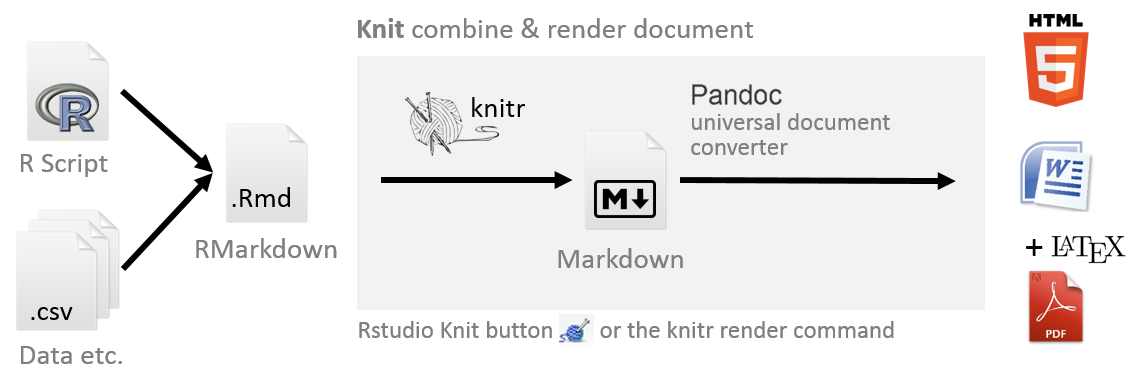
\includegraphics{img/processRStudio.png}
\caption{}
\end{figure}

\begin{center}\rule{0.5\linewidth}{\linethickness}\end{center}

\begin{figure}
\centering

\includegraphics{img/hex/rmarkdown-200x232.png}
\caption{}
\end{figure}

\begin{quote}
\texttt{R\ Markdown} documents are fully reproducible. Use a productive
\textbf{notebook} interface to weave together narrative text and code to
produce elegantly formatted output. Use multiple languages including R,
Python, and SQL \citep{R-rmarkdown}.
\end{quote}

\begin{figure}
\centering

\includegraphics{img/hex/knitr-200x232.png}
\caption{}
\end{figure}

\begin{quote}
\texttt{knitr} is an engine for dynamic report generation with R. It is
a package in the statistical programming language R that enables
integration of \textbf{R code} into LaTeX, LyX, HTML, Markdown,
AsciiDoc, and \textbf{text} documents \citep{R-knitr}.
\end{quote}

\chapter{Install R}\label{install-r}

\begin{figure}
\centering

\includegraphics{img/Rlogo_200.png}
\caption{}
\end{figure}

Here is where we talk about installing R.

\begin{center}\rule{0.5\linewidth}{\linethickness}\end{center}

\section{First Time Installation}\label{first-time-installation}

\begin{quote}
Go to: \href{http://www.r-project.org}{www.r-project.org}
\end{quote}

Get the latest released version of FREE \textbf{Base} \(R\) from
\(CRAN\)

\begin{itemize}
\tightlist
\item
  Choose a mirror close to your geographical location
\item
  Select \textbf{base} \(R\) for your computer \emph{(Windows, Mac,
  ect.)}
\item
  The defaults are good\ldots{}don't change them\ldots{}just keep
  clicking \emph{`Next'}
\end{itemize}

\begin{center}\rule{0.5\linewidth}{\linethickness}\end{center}

\section{Update Regularly}\label{update-regularly}

\chapter{Install R Studio}\label{install-r-studio}

\begin{figure}
\centering

\includegraphics{img/rstudiosticker.png}
\caption{}
\end{figure}

Here is where we talk about installing R Studio.

\begin{center}\rule{0.5\linewidth}{\linethickness}\end{center}

\section{First Time Installation}\label{first-time-installation-1}

\begin{quote}
Go to: \href{http://www.rstudio.com}{www.rstudio.com}
\end{quote}

Get the latest version of the FREE Open Source \textbf{Desktop} Edition
of R Studio

\begin{itemize}
\tightlist
\item
  The defaults are good\ldots{}don't change them\ldots{}just keep
  clicking \emph{`Next'}
\end{itemize}

\begin{center}\rule{0.5\linewidth}{\linethickness}\end{center}

\section{Update Regularly}\label{update-regularly-1}

\begin{center}\rule{0.5\linewidth}{\linethickness}\end{center}

\section{Panel Layout}\label{panel-layout}

\chapter{Install TeX}\label{install-tex}

\begin{figure}
\centering

\includegraphics{img/latex.png}
\caption{}
\end{figure}

Here is where we talk about installing Tex.

\begin{center}\rule{0.5\linewidth}{\linethickness}\end{center}

\section{\texorpdfstring{Use \texttt{tinytex}
package}{Use tinytex package}}\label{use-tinytex-package}

\begin{center}\rule{0.5\linewidth}{\linethickness}\end{center}

\section{\texorpdfstring{Mac - use
\texttt{MacTeX}}{Mac - use MacTeX}}\label{mac---use-mactex}

\begin{quote}
Go to: \url{http://tug.org/mactex/}
\end{quote}

\begin{itemize}
\tightlist
\item
  Download (5+ min) to a folder and them double click on the \textbf{PKG
  file}
\item
  Follow the installation instructions.
\item
  You don't need to open anything after MacTeX is finished installing.
\end{itemize}

\begin{center}\rule{0.5\linewidth}{\linethickness}\end{center}

\section{\texorpdfstring{Windows - use
\texttt{MikTeX}}{Windows - use MikTeX}}\label{windows---use-miktex}

\begin{quote}
Go to: \url{http://miktex.org/download}
\end{quote}

\begin{itemize}
\tightlist
\item
  Pick the latest version of the \textbf{Net Installer}, not the Basic!
\item
  You need the full version 64-bit is better, if you have a 64-bit
  machine
\item
  When your download is complete, run the downloaded installer.
\item
  Windows may ask you if you want to \emph{``allow this app from an
  unknown publisher to make changes to your PC''}. If it does, make sure
  to click \textbf{Yes!}
\item
  This is the slowest part\ldots{}
\end{itemize}

\chapter{Install Packages}\label{install-packages}

We describe packages and their management

\begin{center}\rule{0.5\linewidth}{\linethickness}\end{center}

\section{What are packages}\label{what-are-packages}

\begin{quote}
\textbf{R packages} are collections of functions and data sets developed
by the community. They increase the power of \textbf{R} by improving
existing base \textbf{R} functionalities, or by adding new ones.
\end{quote}

More information may be found here:
\url{https://www.datacamp.com/community/tutorials/r-packages-guide}

\begin{center}\rule{0.5\linewidth}{\linethickness}\end{center}

\section{Installing packages (via the user
interface)}\label{installing-packages-via-the-user-interface}

\begin{quote}
You only need to INSTALL packages ONCE per computer.
\end{quote}

In \textbf{R Stuido}:

\begin{enumerate}
\def\labelenumi{\arabic{enumi}.}
\tightlist
\item
  Click on the \textbf{Packages} tab the panel with the most tabs
\item
  Click on the word \textbf{Instsall} just under and to the left of the
  tab
\item
  In the \textbf{Packages} box, type in the name of the packages you
  would like to download. You can do several at once, just seperate them
  with multiple spaces or a comma.
\end{enumerate}

\emph{Note: Leave the installation library path as the default. Also,
make sure the box for `Installing dependencies' is checked.}

\begin{figure}
\centering
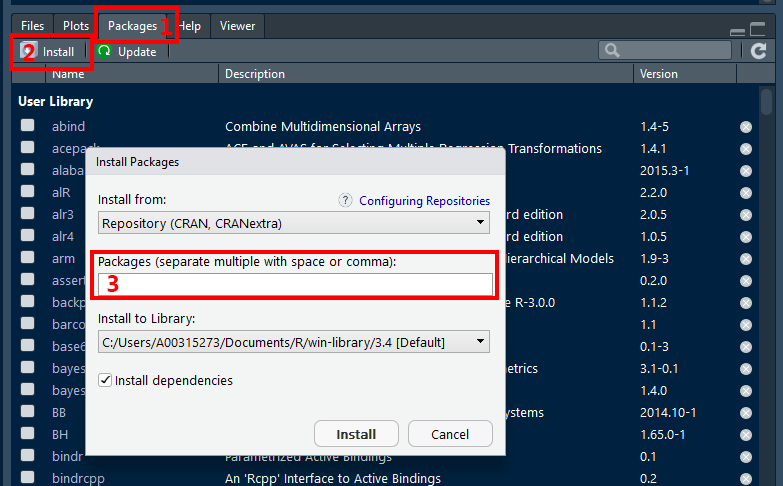
\includegraphics{img/Install_Package_Screenshot.png}
\caption{}
\end{figure}

You can \emph{copy-and-paste} the following list into the box (labeled
3) to load the packages that we use most commonly all at once.

\begin{quote}
tidyverse, furniture, pander, stargazer, texreg, xtable, RColorBrewer,
gghighlight, ggthemes, ggfortify, ggalt, ggExtra, GGally, ggeffects,
corrplot, gpairs, gridextra, likert, vcd, scales, cowplot, yarrr, psych,
polycor, corpcor, sjlabelled, sjPlot, sjmisc, sjstats, Hmisc, labelled,
afex, emmeans, corpcor, multicomp, multcompView, car, effects,
predictmean, nlme, lme4, lmerTest, HLMdiag, geepack, gee, gee4, optimx,
MuMIn, lavaan, OpenMx, sem, semPlot, randomForest, randomForestSRC,
ggRandomForests, party, partykit, mgcv, glmnet, survival, caret,
bookdown, blogdown, tidytex, xaringan, REDCapR, redcapAPI, devtools,
testthat, roxygen2
\end{quote}

When you click the \textbf{Install} buttom, a smaller window may asks if
you would like to re-start \(R\) prior to installing, choose ``no'' and
manually close and open the \(R Studio\) program once all packages have
been downloaded, unpacked, and checked. This may take a few minutes,
especially if you have selected multiple packages.

\begin{quote}
See Chapter 6 for more information on how to install packages another
way (via syntax code), as well as website links for each package.
\end{quote}

\begin{center}\rule{0.5\linewidth}{\linethickness}\end{center}

\section{Updating packages}\label{updating-packages}

\chapter{Loading Packages}\label{loading-packages}

\begin{center}\rule{0.5\linewidth}{\linethickness}\end{center}

\begin{quote}
While you only need to INSTALL a package ONCE per computer, you will
need to LOAD each package in EVERY SESSION you want to use them in.
\end{quote}

\section{\texorpdfstring{LOAD packages (via \(R\)
code)}{LOAD packages (via R code)}}\label{load-packages-via-r-code}

Please don't get confused: \texttt{library()} is the command used to
\textbf{load a package}, and it refers to the \textbf{place} where the
package is contained, usually a folder on your computer, while a package
is the collection of functions bundled conveniently.

Maybe it can help a quote from \textbf{Hadley Wickham}, Chief data
scientist at RStudio, and instructor of the \emph{``Writing functions in
R''} DataCamp course (December 8, 2014):

\begin{quote}
``a package is a like a book, a library is like a library; you use
\texttt{library()} to check a package out of the library''
\end{quote}

\begin{Shaded}
\begin{Highlighting}[]
\KeywordTok{library}\NormalTok{(tidyverse)}
\end{Highlighting}
\end{Shaded}

Here is link to an AWSOME
\href{http://datacamp-community.s3.amazonaws.com/e63a8f6b-2aa3-4006-89e0-badc294b179c}{`cheat
sheet' for begginers working with the \texttt{tidyverse} package}. I
highly suggest checking it out.

More `cheat sheets' are available under the ``Help'' menu option in
\textbf{R Studio}

\chapter{Commonly Used Packages}\label{commonly-used-packages}

Here is where we talk about usefull packages\ldots{}

\begin{center}\rule{0.5\linewidth}{\linethickness}\end{center}

A curated list of awesome \(R\) packages and tools:
\url{https://awesome-r.com/}

\section{\texorpdfstring{The Tidy-Universe from
\(R Studio\)}{The Tidy-Universe from R Studio}}\label{the-tidy-universe-from-r-studio}

\begin{Shaded}
\begin{Highlighting}[]
\KeywordTok{install.packages}\NormalTok{(}\StringTok{"tidyverse"}\NormalTok{)}
\end{Highlighting}
\end{Shaded}

\begin{quote}
The \texttt{tidyverse}
\href{https://www.tidyverse.org/}{(www.tidyverse.org)} is an opinionated
\textbf{collection of \(R\) packages} designed for data science. All
packages share an underlying design philosophy, grammar, and data
structures.
\end{quote}

\subsection{Core}\label{core}

The core tidyverse includes the packages that you are likely to use in
everyday data analyses. As of \texttt{tidyverse\ 1.2.0}, the following
packages are included in the core tidyverse:

\begin{Shaded}
\begin{Highlighting}[]
\KeywordTok{library}\NormalTok{(tidyverse)}
\end{Highlighting}
\end{Shaded}

\begin{longtable}[]{@{}rl@{}}
\toprule
website & description\tabularnewline
\midrule
\endhead
\href{https://dplyr.tidyverse.org/}{\texttt{dplyr}} & A Grammar of Data
Manipulation\tabularnewline
\href{https://forcats.tidyverse.org/}{\texttt{forcats}} & Tools for
Working with Categorical Variables \emph{(Factors)}\tabularnewline
\href{https://ggplot2.tidyverse.org/}{\texttt{ggplot2}} & Create Elegant
Data Visualisations Using the Grammar of Graphics\tabularnewline
\href{https://purrr.tidyverse.org/}{\texttt{purrr}} & Functional
Programming Tools\tabularnewline
\href{https://readr.tidyverse.org/}{\texttt{readr}} & Read Rectangular
Text Data\tabularnewline
\href{https://stringr.tidyverse.org/}{\texttt{stringr}} & Simple,
Consistent Wrappers for Common String Operations
\emph{(Text)}\tabularnewline
\href{https://tibble.tidyverse.org/}{\texttt{tibble}} & Simple Data
Frames\tabularnewline
\href{https://tidyr.tidyverse.org/}{\texttt{tidyr}} & Easily Tidy Data
with \texttt{spread()} and \texttt{gather()} Functions\tabularnewline
\bottomrule
\end{longtable}

\subsection{Supplemental}\label{supplemental}

The tidyverse also includes many other packages with more specialised
usage. They are not loaded automatically with
\texttt{library(tidyverse)}, so you'll need to load each one with its
own call to \texttt{library()}.

\begin{Shaded}
\begin{Highlighting}[]
\KeywordTok{library}\NormalTok{(haven) }\CommentTok{# example...may replace with any individual package name}
\end{Highlighting}
\end{Shaded}

\begin{longtable}[]{@{}rl@{}}
\toprule
website & description\tabularnewline
\midrule
\endhead
\href{https://github.com/tidymodels/broom}{\texttt{broom}} & Convert
Statistical Analysis Objects into Tidy Tibbles\tabularnewline
\href{https://haven.tidyverse.org/}{\texttt{haven}} & Import and Export
\textbf{SPSS}, \textbf{Stata} and \textbf{SAS} Files\tabularnewline
\href{https://github.com/tidyverse/hms}{\texttt{hms}} & Pretty Time of
Day\tabularnewline
\href{https://lubridate.tidyverse.org/}{\texttt{lubridate}} & Make
Dealing with Dates a Little Easier\tabularnewline
\href{https://magrittr.tidyverse.org/}{\texttt{magrittr}} & A
Forward-Pipe Operator for \textbf{\(R\)}\tabularnewline
\href{https://github.com/tidyverse/glue}{\texttt{glue}} & Interpreted
String Literals\tabularnewline
\href{https://readxl.tidyverse.org/}{\texttt{readxl}} & Read
\textbf{Excel} Files\tabularnewline
\href{https://tibble.tidyverse.org/}{\texttt{tibble}} & Simple Data
Frames\tabularnewline
\bottomrule
\end{longtable}

\begin{center}\rule{0.5\linewidth}{\linethickness}\end{center}

\section{\texorpdfstring{Groups of Individual Packages on
\(CRAN\)}{Groups of Individual Packages on CRAN}}\label{groups-of-individual-packages-on-cran}

\begin{center}\rule{0.5\linewidth}{\linethickness}\end{center}

\subsection{Creating Tables}\label{creating-tables}

\begin{longtable}[]{@{}rl@{}}
\toprule
website & description\tabularnewline
\midrule
\endhead
\href{http://tysonbarrett.com/furniture/}{\texttt{furniture}} & Tables
for Quantitative Scientists\tabularnewline
\href{https://rapporter.github.io/pander/}{\texttt{pander}} & An R
`Pandoc' Writer (makes tables look nice)\tabularnewline
\href{https://www.jakeruss.com/cheatsheets/stargazer/}{\texttt{stargazer}}
& Well-Formatted Regression and Summary Statistics Tables\tabularnewline
\href{https://diffuseprior.wordpress.com/2013/01/20/texreg-a-package-for-beautiful-and-easily-customizable-latex-regression-tables-from-r/}{\texttt{texreg}}
& Conversion of R Regression Output to LaTeX or HTML
Tables\tabularnewline
\href{https://cran.r-project.org/web/packages/xtable/vignettes/xtableGallery.pdf}{\texttt{xtable}}
& Export Tables to LaTeX or HTML\tabularnewline
\bottomrule
\end{longtable}

\begin{center}\rule{0.5\linewidth}{\linethickness}\end{center}

\subsection{Visualization}\label{visualization}

\begin{longtable}[]{@{}rl@{}}
\toprule
website & description\tabularnewline
\midrule
\endhead
\href{https://data.library.virginia.edu/setting-up-color-palettes-in-r/}{\texttt{RColorBrewer}}
& Color Palettes\tabularnewline
\href{https://github.com/yutannihilation/gghighlight}{\texttt{gghighlight}}
& Highlight Lines and Points in \texttt{ggplot2}\tabularnewline
\href{https://www.ggplot2-exts.org/ggthemes.html}{\texttt{ggthemes}} &
Extra Themes, Scales, and Geoms for \texttt{ggplot2}\tabularnewline
\href{https://www.ggplot2-exts.org/ggExtra.html}{\texttt{ggExtra}} & Add
Marginal Histograms to \texttt{ggplot2}, and More \texttt{ggplot2}
Enhancements\tabularnewline
\href{https://github.com/sinhrks/ggfortify}{\texttt{ggfortify}} & Data
Visualization Tools for Statistical Analysis Results\tabularnewline
\href{https://github.com/hrbrmstr/ggalt}{\texttt{ggalt}} & Lots of
extras for \texttt{ggplot2}\tabularnewline
\href{https://ggobi.github.io/ggally/\#canonical_correlation_analysis}{\texttt{GGally}}
& Extension to \texttt{ggplot2}\tabularnewline
\href{https://rstudio-pubs-static.s3.amazonaws.com/240657_5157ff98e8204c358b2118fa69162e18.html}{\texttt{corrplot}}
& Visualization of a Correlation Matrix\tabularnewline
\texttt{gpairs} & The Generalized Pairs Plot\tabularnewline
\href{https://cran.r-project.org/web/packages/egg/vignettes/Ecosystem.html}{\texttt{gridextra}}
& Miscellaneous Functions for ``Grid'' Graphics\tabularnewline
\href{https://github.com/jbryer/likert}{\texttt{likert}} & Analysis and
Visualization Likert Items\tabularnewline
\href{http://www.datavis.ca/courses/VCD/vcd-tutorial.pdf}{\texttt{vcd}}
& Visualizing Categorical Data\tabularnewline
\href{https://github.com/r-lib/scales}{\texttt{scales}} & Scale
Functions for Visualization\tabularnewline
\href{https://cran.r-project.org/web/packages/cowplot/vignettes/introduction.html}{\texttt{cowplot}}
& Streamlined Plot Theme \& Annotations for
\texttt{ggplot2}\tabularnewline
\href{https://ndphillips.github.io/piratesguide.html}{\texttt{yarrr}} &
The Pirate's Guide to \(R\)\tabularnewline
\bottomrule
\end{longtable}

\begin{center}\rule{0.5\linewidth}{\linethickness}\end{center}

\subsection{Generally Handy}\label{generally-handy}

\begin{longtable}[]{@{}rl@{}}
\toprule
website & description\tabularnewline
\midrule
\endhead
\texttt{polycor} & Polychoric and Polyserial Correlations\tabularnewline
\href{http://personality-project.org/r/psych/}{\texttt{psych}} &
Psychological or Psychometric Procedures\tabularnewline
\href{http://strimmerlab.org/software/corpcor/}{\texttt{corpcor}} &
Covariance and (Partial) Correlation\tabularnewline
\href{https://strengejacke.github.io/sjlabelled/}{\texttt{sjlabelled}} &
Labelled Data Utility Functions\tabularnewline
\href{http://www.strengejacke.de/sjPlot/}{\texttt{sjPlot}} & Data
Visualization for Statistics in Social Science\tabularnewline
\href{http://www.strengejacke.de/sjmisc/}{\texttt{sjmisc}} & Data and
Variable Transformation Functions\tabularnewline
\href{http://www.strengejacke.de/sjstats/}{\texttt{sjstats}} &
Convenient Functions for Common Statistical Computations\tabularnewline
\href{http://biostat.mc.vanderbilt.edu/wiki/Main/Hmisc}{\texttt{Hmisc}}
& Harrell Miscellaneous\tabularnewline
\href{https://github.com/larmarange/labelled}{\texttt{labelled}} &
Manipulating Labelled Data\tabularnewline
\bottomrule
\end{longtable}

\begin{center}\rule{0.5\linewidth}{\linethickness}\end{center}

\subsection{t-Tests, ANOVA, and RM
ANOVA}\label{t-tests-anova-and-rm-anova}

\begin{longtable}[]{@{}rl@{}}
\toprule
website & description\tabularnewline
\midrule
\endhead
\href{https://github.com/singmann/afex}{\texttt{afex}} & Analysis of
Factorial Experiments\tabularnewline
\href{https://github.com/rvlenth/emmeans}{\texttt{emmeans}} & Estimated
Marginal Means, aka Least-Squares Means\tabularnewline
\href{http://multcomp.r-forge.r-project.org/}{\texttt{multicomp}} &
Simultaneous Inference in General Parametric Models\tabularnewline
\texttt{multcompView} & Visualizations of Paired
Comparisons\tabularnewline
\bottomrule
\end{longtable}

\begin{center}\rule{0.5\linewidth}{\linethickness}\end{center}

\subsection{Regression (ML, GLM)}\label{regression-ml-glm}

\begin{longtable}[]{@{}rl@{}}
\toprule
website & description\tabularnewline
\midrule
\endhead
\href{https://www.statmethods.net/stats/rdiagnostics.html}{\texttt{car}}
& Companion to Applied Regression\tabularnewline
\href{https://www.jstatsoft.org/article/view/v008i15/effect-displays-revised.pdf}{\texttt{effects}}
& Effect Displays for Linear, Generalized Linear, and Other
Models\tabularnewline
\texttt{predictmeans} & Calculate Predicted Means for Linear
Models\tabularnewline
\bottomrule
\end{longtable}

\begin{center}\rule{0.5\linewidth}{\linethickness}\end{center}

\subsection{Multilevel Models (MLM, HLM,
GEE)}\label{multilevel-models-mlm-hlm-gee}

\begin{longtable}[]{@{}rl@{}}
\toprule
website & description\tabularnewline
\midrule
\endhead
\href{http://davidakenny.net/papers/k\&h/MLM_R.pdf}{\texttt{nlme}} &
Linear and Nonlinear Mixed Effects Models\tabularnewline
\href{https://github.com/lme4/lme4/}{\texttt{lme4}} & Linear
Mixed-Effects Models\tabularnewline
\href{https://github.com/runehaubo/lmerTestR}{\texttt{lmerTest}} & Tests
in Linear Mixed Effects Models\tabularnewline
\href{https://github.com/aloy/HLMdiag}{\texttt{HLMdiag}} & Diagnostic
Tools for Hierarchical (Multilevel) Linear Models\tabularnewline
\href{https://cran.r-project.org/web/packages/geepack/vignettes/geepack-manual.pdf}{\texttt{geepack}}
& Generalized Estimating Equation Package\tabularnewline
\href{https://cran.r-project.org/web/packages/gee/gee.pdf}{\texttt{gee}}
& Generalized Estimation Equation Solver\tabularnewline
\href{https://github.com/ypan1988/gee4}{\texttt{gee4}} & Generalised
Estimating Equations (GEE/WGEE)\tabularnewline
\href{file:///C:/Users/A00315273/Downloads/v43i09.pdf}{\texttt{optimx}}
& A Replacement and Extension of the \texttt{optim()}
Function\tabularnewline
\href{https://sites.google.com/site/rforfishandwildlifegrads/home/mumin_usage_examples}{\texttt{MuMIn}}
& Multi-Model Inference\tabularnewline
\bottomrule
\end{longtable}

\begin{center}\rule{0.5\linewidth}{\linethickness}\end{center}

\subsection{Structural Equation Modeling
(SEM)}\label{structural-equation-modeling-sem}

\begin{longtable}[]{@{}rl@{}}
\toprule
website & description\tabularnewline
\midrule
\endhead
\href{http://lavaan.org}{\texttt{lavaan}} & Latent Variable
Analysis\tabularnewline
\href{https://openmx.ssri.psu.edu/}{\texttt{OpenMx}} & Extended
Structural Equation Modelling\tabularnewline
\href{https://www.methodsconsultants.com/tutorial/structural-equation-models-using-the-sem-package-in-r/}{\texttt{sem}}
& Structural Equation Modelling\tabularnewline
\href{http://sachaepskamp.com/semPlot/examples}{\texttt{semPlot}} & Path
Diagrams and Visual Analysis of Various SEM Packages'
Output\tabularnewline
\bottomrule
\end{longtable}

\begin{center}\rule{0.5\linewidth}{\linethickness}\end{center}

\subsection{Random Forests}\label{random-forests}

\begin{longtable}[]{@{}rl@{}}
\toprule
website & description\tabularnewline
\midrule
\endhead
\href{https://www.guru99.com/r-random-forest-tutorial.html}{\texttt{randomForest}}
& Random Forests for Classification and Regression\tabularnewline
\href{http://www.riptutorial.com/r/example/13086/random-forest-survival-analysis-with-randomforestsrc}{\texttt{randomForestSRC}}
& for Survival, Regression, and Classification\tabularnewline
\href{https://arxiv.org/pdf/1612.08974.pdf}{\texttt{ggRandomForests}} &
Visually Exploring Random Forests\tabularnewline
\href{http://party.r-forge.r-project.org/}{\texttt{party}} & A
Laboratory for Recursive Partytioning\tabularnewline
\href{}{\texttt{partykit}} & A Toolkit for Recursive
Partytioning\tabularnewline
\bottomrule
\end{longtable}

\begin{center}\rule{0.5\linewidth}{\linethickness}\end{center}

\subsection{Other Models}\label{other-models}

\begin{longtable}[]{@{}rl@{}}
\toprule
website & description\tabularnewline
\midrule
\endhead
\href{https://people.maths.bris.ac.uk/~sw15190/mgcv/tampere/mgcv.pdf}{\texttt{mgcv}}
& Mixed GAM Computation Vehicle with Automatic Smoothness
Estimation\tabularnewline
\href{https://web.stanford.edu/~hastie/glmnet/glmnet_alpha.html}{\texttt{glmnet}}
& Lasso and Elastic-Net Regularized Generalized Linear
Models\tabularnewline
\href{https://github.com/therneau/survival}{\texttt{survival}} &
Survival Analysis\tabularnewline
\href{https://topepo.github.io/caret/index.html}{\texttt{caret}} &
Classification and Regression Training\tabularnewline
\bottomrule
\end{longtable}

\begin{center}\rule{0.5\linewidth}{\linethickness}\end{center}

\subsection{Reproducibility and
Reporting}\label{reproducibility-and-reporting}

\begin{longtable}[]{@{}rl@{}}
\toprule
website & description\tabularnewline
\midrule
\endhead
\href{https://bookdown.org/}{\texttt{bookdown}} & Authoring Books and
Technical Documents\tabularnewline
\href{https://bookdown.org/yihui/blogdown/}{\texttt{blogdown}} & Create
Blogs and Websites\tabularnewline
\href{https://yihui.name/tinytex/}{\texttt{tidytex}} & Helper
Functionsfor \(TeX Live\), Compile \(LaTeX\) Documents\tabularnewline
\href{https://github.com/yihui/xaringan}{\texttt{xaringan}} &
Presentation Ninja\tabularnewline
\bottomrule
\end{longtable}

\emph{Note: \texttt{slidify} \& \texttt{ReportRs} have been removed from
\(CRAN\)}

\begin{center}\rule{0.5\linewidth}{\linethickness}\end{center}

\subsection{REDCap Interface}\label{redcap-interface}

\begin{longtable}[]{@{}rl@{}}
\toprule
website & description\tabularnewline
\midrule
\endhead
\href{https://github.com/nutterb/redcapAPI/wiki}{\texttt{redcapAPI}} &
Interface to \(REDCap\)\tabularnewline
\href{https://github.com/OuhscBbmc/REDCapR}{\texttt{REDCapR}} &
Interaction Between \(R\) and \(REDCap\)\tabularnewline
\bottomrule
\end{longtable}

\begin{center}\rule{0.5\linewidth}{\linethickness}\end{center}

\subsection{Creating Your Own
Packages}\label{creating-your-own-packages}

\begin{longtable}[]{@{}rl@{}}
\toprule
website & description\tabularnewline
\midrule
\endhead
\href{https://github.com/r-lib/devtools}{\texttt{devtools}} & Tools to
Make Developing \(R\) Packages Easier\tabularnewline
\href{https://github.com/r-lib/testthat}{\texttt{testthat}} & Unit
Testing for \(R\)\tabularnewline
\href{https://cran.r-project.org/web/packages/roxygen2/vignettes/roxygen2.html}{\texttt{roxygen2}}
& In-Line Documentation for \(R\)\tabularnewline
\bottomrule
\end{longtable}

\begin{center}\rule{0.5\linewidth}{\linethickness}\end{center}

\section{\texorpdfstring{Install All the \(CRAN\) Packages at Once (via
syntax
code)}{Install All the CRAN Packages at Once (via syntax code)}}\label{install-all-the-cran-packages-at-once-via-syntax-code}

Review the list of all the packages above:

\begin{Shaded}
\begin{Highlighting}[]
\NormalTok{package_list_tables}
\end{Highlighting}
\end{Shaded}

\begin{verbatim}
[1] "furniture" "pander"    "stargazer" "texreg"    "xtable"   
\end{verbatim}

\begin{Shaded}
\begin{Highlighting}[]
\NormalTok{package_list_visual}
\end{Highlighting}
\end{Shaded}

\begin{verbatim}
 [1] "RColorBrewer" "gghighlight"  "ggthemes"     "ggfortify"   
 [5] "ggalt"        "ggExtra"      "GGally"       "ggeffects"   
 [9] "corrplot"     "gpairs"       "gridextra"    "likert"      
[13] "vcd"          "scales"       "cowplot"      "yarrr"       
\end{verbatim}

\begin{Shaded}
\begin{Highlighting}[]
\NormalTok{package_list_general}
\end{Highlighting}
\end{Shaded}

\begin{verbatim}
[1] "psych"      "polycor"    "corpcor"    "sjlabelled" "sjPlot"    
[6] "sjmisc"     "sjstats"    "Hmisc"      "labelled"  
\end{verbatim}

\begin{Shaded}
\begin{Highlighting}[]
\NormalTok{package_list_anova}
\end{Highlighting}
\end{Shaded}

\begin{verbatim}
[1] "afex"         "emmeans"      "corpcor"      "multicomp"   
[5] "multcompView"
\end{verbatim}

\begin{Shaded}
\begin{Highlighting}[]
\NormalTok{package_list_regression}
\end{Highlighting}
\end{Shaded}

\begin{verbatim}
[1] "car"          "effects"      "predictmeans"
\end{verbatim}

\begin{Shaded}
\begin{Highlighting}[]
\NormalTok{package_list_multilevel}
\end{Highlighting}
\end{Shaded}

\begin{verbatim}
[1] "nlme"     "lme4"     "lmerTest" "HLMdiag"  "geepack"  "gee"     
[7] "gee4"     "optimx"   "MuMIn"   
\end{verbatim}

\begin{Shaded}
\begin{Highlighting}[]
\NormalTok{package_list_sem}
\end{Highlighting}
\end{Shaded}

\begin{verbatim}
[1] "lavaan"  "OpenMx"  "sem"     "semPlot"
\end{verbatim}

\begin{Shaded}
\begin{Highlighting}[]
\NormalTok{package_list_forest}
\end{Highlighting}
\end{Shaded}

\begin{verbatim}
[1] "randomForest"    "randomForestSRC" "ggRandomForests" "party"          
[5] "partykit"       
\end{verbatim}

\begin{Shaded}
\begin{Highlighting}[]
\NormalTok{package_list_models}
\end{Highlighting}
\end{Shaded}

\begin{verbatim}
[1] "mgcv"     "glmnet"   "survival" "caret"   
\end{verbatim}

\begin{Shaded}
\begin{Highlighting}[]
\NormalTok{package_list_report}
\end{Highlighting}
\end{Shaded}

\begin{verbatim}
[1] "bookdown" "blogdown" "tidytex"  "xaringan" "slidify"  "ReportRs"
\end{verbatim}

\begin{Shaded}
\begin{Highlighting}[]
\NormalTok{package_list_redcap}
\end{Highlighting}
\end{Shaded}

\begin{verbatim}
[1] "REDCapR"   "redcapAPI"
\end{verbatim}

\begin{Shaded}
\begin{Highlighting}[]
\NormalTok{package_list_package}
\end{Highlighting}
\end{Shaded}

\begin{verbatim}
[1] "devtools" "testthat" "roxygen2"
\end{verbatim}

Get all the packages from \(CRAN\) \emph{(updates if new version
available)}:

\begin{Shaded}
\begin{Highlighting}[]
\KeywordTok{install.packages}\NormalTok{(}\KeywordTok{c}\NormalTok{(}\StringTok{"tidyverse"}\NormalTok{,}
\NormalTok{                   package_list_tables,}
\NormalTok{                   package_list_visual,}
\NormalTok{                   package_list_general,}
\NormalTok{                   package_list_anova,}
\NormalTok{                   package_list_regression,}
\NormalTok{                   package_list_multilevel,}
\NormalTok{                   package_list_sem,}
\NormalTok{                   package_list_forest,}
\NormalTok{                   package_list_models,}
\NormalTok{                   package_list_report,}
\NormalTok{                   package_list_redcap,}
\NormalTok{                   package_list_package))}
\end{Highlighting}
\end{Shaded}

\begin{center}\rule{0.5\linewidth}{\linethickness}\end{center}

\section{\texorpdfstring{Other Developmental non-\(CRAN\) Packages on
\(GitHub\)}{Other Developmental non-CRAN Packages on GitHub}}\label{other-developmental-non-cran-packages-on-github}

First, make sure you have the \texttt{devtools} package installed on
your computer \emph{(hint: its in the \texttt{package\_list\_package}
list above)}.

\begin{Shaded}
\begin{Highlighting}[]
\KeywordTok{install.packages}\NormalTok{(}\StringTok{"devtools"}\NormalTok{)}
\end{Highlighting}
\end{Shaded}

\begin{center}\rule{0.5\linewidth}{\linethickness}\end{center}

\subsection{\texorpdfstring{Templates for writing tutorials, practicals
or examination papers with
\(R Markdown\)}{Templates for writing tutorials, practicals or examination papers with R Markdown}}\label{templates-for-writing-tutorials-practicals-or-examination-papers-with-r-markdown}

\texttt{unilur} is a \(R\) package to help writing tutorials, practicals
or examination papers with \(R Markdown\).

With \texttt{unilur} you can render the following outputs from a single
rmarkdown file:

\begin{itemize}
\item
  the exam or tutorial questions (answers remaining hidden) as a PDF or
  HTML file.
\item
  the exam or tutorial questions with sample answers as a PDF or HTML
  file.
\end{itemize}

In addition, you will be able to:

\begin{itemize}
\item
  Create coloured boxes to highlight some markdown or R content.
\item
  Create examination papers with

  \begin{itemize}
  \tightlist
  \item
    multiple choice questions
  \item
    a candidate identification form
  \item
    dotted lines placeholders to fill in answers
  \end{itemize}
\item
  Create a new \(R Markdown\) file with solution chunks replaced by
  empty ones.
\end{itemize}

\begin{quote}
Website: \href{https://github.com/koncina/unilur}{GitHub -
\texttt{unilur}}
\end{quote}

\begin{quote}
Tutorial:
\href{http://eric.koncina.eu/posts/introducing-the-unilur-rmarkdown-template/}{blog
post - \texttt{unilur}}
\end{quote}

\begin{Shaded}
\begin{Highlighting}[]
\NormalTok{devtools}\OperatorTok{::}\KeywordTok{install_github}\NormalTok{(}\StringTok{"koncina/unilur"}\NormalTok{)}
\end{Highlighting}
\end{Shaded}

\begin{center}\rule{0.5\linewidth}{\linethickness}\end{center}

\subsection{\texorpdfstring{Prepare APA journal articles with
\(R Markdown\)}{Prepare APA journal articles with R Markdown}}\label{prepare-apa-journal-articles-with-r-markdown}

\texttt{papaja} is a \(R\) package in the making including a
\(R Markdown\) template that can be used with (or without) \textbf{\(R\)
Studio} to produce documents, which conform to the \textbf{American
Psychological Association (APA)} manuscript guidelines (6th Edition).
The package uses the \(LaTeX\) document class \texttt{apa6} and a
.docx-reference file, so you can create PDF documents, or Word documents
if you have to. Moreover, papaja supplies \(R\) functions that
facilitate reporting results of your analyses in accordance with APA
guidelines.

\texttt{papaja} has not yet been submitted to \(CRAN\) because it is
under active development. Currently, there are still a couple of loose
ends they would like to tie up before we release the package to a larger
audience. There are two versions you can install from the \(GitHub\)
website.

\begin{quote}
Website: \href{https://github.com/crsh/papaja}{GitHub - \texttt{papaja}}
\end{quote}

\begin{quote}
Tutorial: \href{https://crsh.github.io/papaja_man/}{eBook -
\texttt{papaja}}
\end{quote}

\begin{Shaded}
\begin{Highlighting}[]
\CommentTok{# Install the stable development verions from GitHub}
\NormalTok{devtools}\OperatorTok{::}\KeywordTok{install_github}\NormalTok{(}\StringTok{"crsh/papaja"}\NormalTok{)}

\CommentTok{# Install the latest development snapshot from GitHub}
\NormalTok{devtools}\OperatorTok{::}\KeywordTok{install_github}\NormalTok{(}\StringTok{"crsh/papaja@devel"}\NormalTok{)}
\end{Highlighting}
\end{Shaded}

\chapter{Kniting Notebooks}\label{kniting-notebooks}

\begin{center}\rule{0.5\linewidth}{\linethickness}\end{center}

\section{Storing all associated
files}\label{storing-all-associated-files}

If you are using any files, such as \emph{datasets} or \emph{images},
they need to be stored in the same folder location as the R Notebook
(\texttt{.Rmd} file).

This folder location must be the \textbf{Working Directory} for the R
Studio session. If you opened your \texttt{.Rmd} notebook file by
double-clicking on its name, then this should be the case.

\begin{center}\rule{0.5\linewidth}{\linethickness}\end{center}

\section{Setting the working
directory}\label{setting-the-working-directory}

To ensure that R Studio knows where to find the files, you can manually
set the \textbf{Working Directory} through the menu:

\begin{itemize}
\tightlist
\item
  Click \texttt{Session}
\item
  Select \texttt{Set\ Working\ Directory} by hovering your mouse over it
\item
  Click on \texttt{To\ Source\ File\ Location}
\end{itemize}

\begin{figure}
\centering
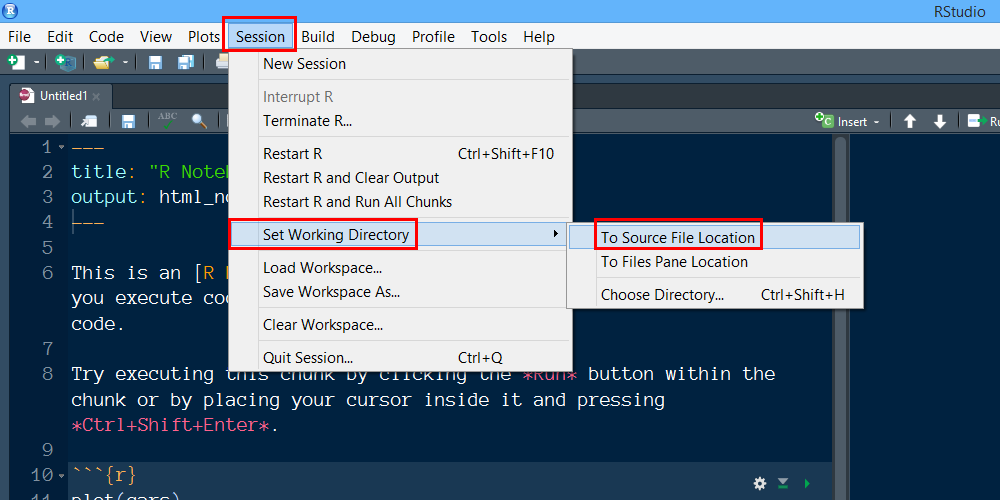
\includegraphics{img/Set_wd_source.png}
\caption{}
\end{figure}

You can double check that you were successful by

\begin{itemize}
\tightlist
\item
  Click on the \texttt{Files} tab in the many-tab panel
\item
  Click on the button with the gear that says \texttt{More}
\item
  Click \texttt{Go\ To\ Working\ Directory}
\end{itemize}

At this point you should see all the files that reside in the folder
location where the open \texttt{.Rmd} files is also saved.

\begin{figure}
\centering
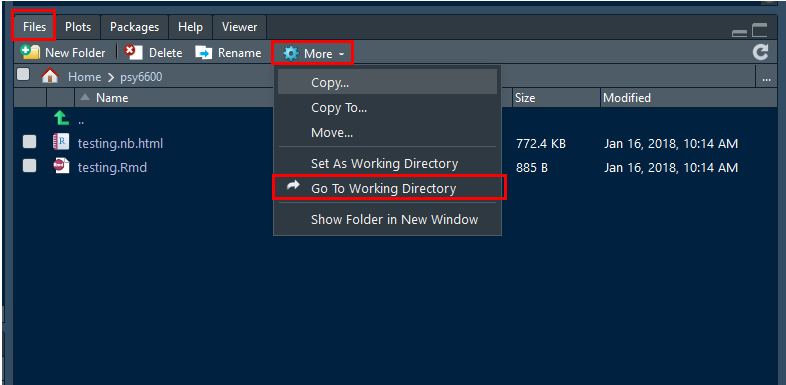
\includegraphics{img/files_goto_wd.png}
\caption{}
\end{figure}

\begin{center}\rule{0.5\linewidth}{\linethickness}\end{center}

\section{\texorpdfstring{Press the \(Knit\)
button}{Press the Knit button}}\label{press-the-knit-button}

\bibliography{book.bib,packages.bib}


\end{document}
